\Chapter{Gesztusok}

\Section{Felismerendő gesztusok}

A szoftver használata közben a prezentáló személy különféle gesztusok segítségével irányíthatja a prezentáció menetét és szintén gesztusok segítségével léphet kapcsolatba a videófolyamon megjelenő virtuális elemekkel. A felhasználó a karjai segítségével valósíthatja meg a mozdulatokat. A gesztusokat az alábbi kategóriákba sorolhatjuk:

\begin{itemize}
	\item \textbf{Sweep}: Egyenes vonalú mozgás, pl.: kézfej végighúzása a képtartományon. A mozgásnak van iránya és két képkocka között megfigyelhető a hossza is.
	\item \textbf{Shift}: Bizonyos virtuális elemek közvetlenül is reagálnak a környezetükben történő mozgásra. Az ilyen elemek az irányukba történő mozgással megegyező irányú mozgással reagálnak. Vagyis a prezentáló személy például a kezei segítségével egyszerűen eltolhatja az adott virtuális elemet. Az ilyen elemeket vezérlő gesztusokat \textit{Shift}-nek nevezhetjük el.
	\item \textbf{Blink}: Az ujjak gyors ökölbe zárása vagy a tenyér széttárásának mozdulata.
	\item \textbf{Drag and Drop}: Bizonyos virtuális elemeket a prezentáló személy képes megfogni, majd odébbhúzni és elengedni. A funkció eléréséhez a prezentálónak az ún. \textit{Drag and Drop} mozgássorozatot kell végrehajtania. Két \textit{Blink} gesztus között szabadon mozgathatja az "elkapott" elemet, majd végül a kívánt helyére teheti azt.
	\item \textbf{Rotation}: A videófolyamon történő örvénylő mozgás, ami akár több ponton is megfigyelhető. Ez lehet például karlendítés, körvonal/ív menti mozgás, tenyerek forgatása.
	\item \textbf{Többpontos kezelés}: A képen lévő összefüggő, nagyobb elmozdulások keresése, \textit{Blob}-ok alapján. Több pont egymáshoz képesti vizsgálata különféle szempontok alapján.
	\item \textbf{Symbol}: Levegőbe leírt szimbólumok, melyek segítségével további funkciókat érhet el a felhasználó.
\end{itemize}

\Section{Képek és vektor mezők}

% A feldolgozás folyamata ábra
% Videófolyam -> két kép kiragadása -> Elmozdulásértékek számítása

A videófolyamon megfigyelhető mozgást a további számítások elvégzéséhez először érzékelnünk kell. Az elmozdulások becslésére az ún. \textit{MotionFlow}/\textit{Optical Flow} technikák tűnnek a legalkalmasabbnak. Egy kiemelkedő és széles körben elterjedt eljárás a Bruce D. Lucas és Takeo Kanade által kidolgozott módszer, melynek implementálása az \textit{OpenCV}-ben is megtalálható.

A Lucas-Kanade módszer dedikált pontok követésére hivatott. Ha a videófomlyaból kiemelünk két képkockát, melyek között az eltelt idő kicsi, a módszer képes megbecsülni a két képkockán elhelyezkedő kijelölt pontok pozíciójának a változását, vagyis megadja a pontok elmozdulás vektorait. A módszer azon a megállapításon alapszik, hogy a videófolyamon egy kijelölt pont és a körülötte lévő pixelek halmaza közel azonos intenzitású $(I)$ a vizsgált időintervallumban. Ha a ponthoz tartozó valós objektum elmozdul a korábbi helyzetéről és az általa képviselt új pont a vizsgálandó terület tartományába esik, akkor a módszer képes becslést adni a vizsgált pont új helyzetére a videófolyamon. A módszer használatánál feltételezzük azt is, hogy a videófolyamon megfigyelhető mozgás viszonylag lassú, vagyis két képkockát vizsgálva az új pont nem eshet kívül a vizsgált pont tartományából. A módszer tetszőleges pontok halmazára alkalmazható. Elsősorban szürkeárnyalatos képekre használatos, de a megfelelő paraméterek megválasztása mellett színes képekre is használható. Színinformációk használata mellett pontosabb eredményt kaphatunk, hiszen ilyenkor egy-egy pont több információt hordozna, viszont a számításigény várhatóan erősen megnövekedne. 

Vegyünk egy pixelt az összehasonlítandó két képkocka egyikéből és jelöljük $I(x,y,t)$-vel, ahol $x,y \in \mathbb{R}$ a pixel pozíciója, $t$ pedig az idő. Tegyük fel, hogy a vizsgálandó pixel $(dx, dy)$ távolsággal elmozdul a következő képkockán megfigyelve $dt$ idővel később. Mivel ezek a pixelek ugyanannak a valós objektumnak a vetületei, ezért feltételezzük, hogy az intenzitásértékük nem változott. Így
\begin{align*}
I(x,y,t) = I(x+dx,y+dy,t+dt)
\end{align*}
Ezután vegyük a jobb oldali kifejezés Taylor-sor közelítését, távolítsuk el a közös kifejezéseket, majd osszunk $dt$-vel. Így a következő egyenletet kapjuk:
\begin{align*}
f_xu+f_yv+f_t=0
\end{align*}
ahol:
\begin{align*}
f_x = \frac{\partial f}{\partial x} &; f_y = \frac{\partial f}{\partial y}\\
u = \frac{dx}{dt} &; v = \frac{dy}{dt}
\end{align*}
A fenti egyenlet \textit{Optical Flow egyenletnek} hívjuk, melyben $f_x$ és $f_y$ kép gradiensek. Hasonlóan, $f_t$ az idő gradiense. De $(u,v)$, vagyis az elmozdulás vektorok ismeretlenek. Ezen kétismeretlenes egyenlet megoldására számos módszer létezik, ezek egyike a \textit{Lucas-Kanade} módszer.

Korábban említettük, hogy a vizsgálandó pont és az őt körülvevő pontok halmazai közel azonos intenzitásértékekkel rendelkeznek a megfigyelés időtartamában. Vegyünk például egy $3 \times 3$-as foltot a vizsgálandó pixel körül. A megállapítás alapján feltételezhetjük, hogy ezen tartományba eső pixelek elmozdulása hasonló lesz. Megkereshetjük az $(f_x,f_y,f_t)$-ket ezekre a pontokra. Így 9 darab kétismeretlenes egyenletet kapunk, amely túlhatározott.

Egy jobb megoldás kapható a \textit{Legkisebb négyzetek módszerének} segítségével. A végső megoldást a következő egyenlettel szemléltethetjük, amely egy két egyeletes-kétismeretlenes probléma:
\begin{align*}
\bmatrix u \\ v \endbmatrix = {\bmatrix \sum_{i}(f_{x_i})^2 & \sum_{i}f_{x_i}f_{y_i}\\ \sum_{i}f_{x_i}f_{y_i} & \sum_{i}(f_{y_i})^2 \endbmatrix}^{-1} \cdot \bmatrix -\sum_{i}f_{x_i}f_{t_i} \\ -\sum_{i}f_{y_i}f_{t_i} \endbmatrix
\end{align*}
Az \textit{OpenCV}-ben található implementáció ún. \textit{Gauss képpiramis}-ok használatával próbálja kiküszöbölni a nagy mozdulatok esetén fellépő hibás eredményeket, vagyis a vizsgálandó képeknek különböző felbontású változatait vizsgálja iteratívan a kisebb felbontástól az eredeti felbontásig haladva. A piramis mélysége tetszőleges, a legkisebb szint egyetlen pixelből is állhat. Kis felbontások mellett a nagyobb mozdulatok könnyebben azonosíthatóak, a piramis szélesebb szintjeihez közelítve, nagyobb felbontások mellett pedig a becslés pontosítása történik. \cite{lucas1981iterative} \cite{bradski2008learning}

\begin{figure}[h]
\centering
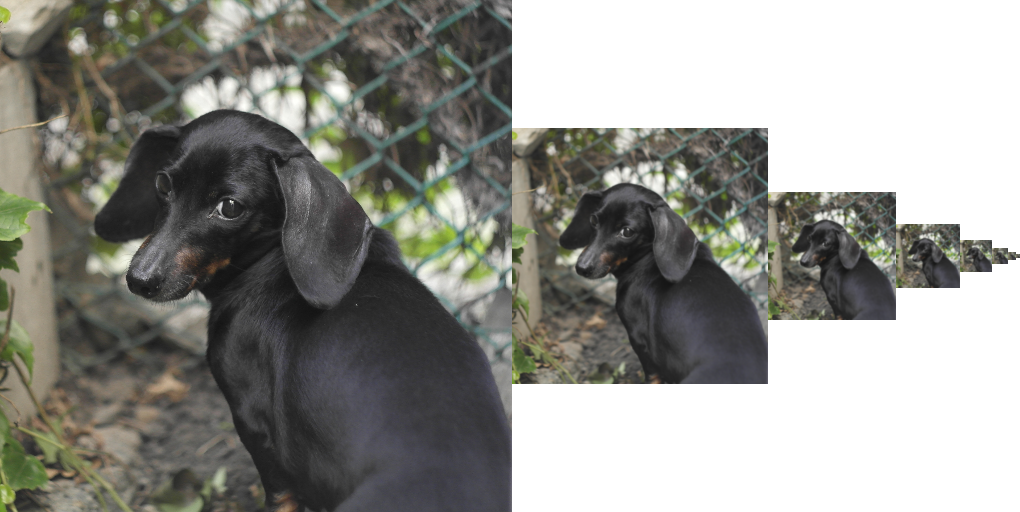
\includegraphics[width=7.65truecm, height=3.84truecm]{images/gauss_pyramid.png}
\caption{Gauss piramis}
\label{fig:gausspyramid}
\end{figure}

A módszer \textit{Spare Optical Flow}-t valósít meg, vagyis egymástól különálló pontokat vizsgál, ellentétben a \textit{Dense Optical Flow} módszerekkel, melyek a teljes kép vizsgálatával számolják ki az elmozdulás vektorokat. \cite{bradski2008learning} Az utóbbi módszerek számításigénye kifejezetten magas. Valós idejű alkalmazás esetén problémákba ütközhetünk gyengébb hardverek esetében. A mozgás valós idejű detektálására a \textit{Spare Optical Flow} módszerek is kielégítő eredményekkel szolgálnak, néhány trükk alkalmazása mellett. Ilyenek például a már említett \textit{kép-piramisok} használata a gyors mozgások pontos követésére és a vizsgálandó pontok kijelölésének a stratégiája is. A pontok kijelöléséhez egy rácsszerkezet használatát gondoltam a legmegfelelőbbnek, ahol a pontok a rács középpontjaiban helyezkednek el. A képtartományt ily módon egyenletesen fedik le a pontok, a további számításokat pedig ehhez tudjuk igazítani.

\Section{Rácspontok kezelése}

Az \textit{Optical Flow} eljárást tetszőleges számú pontra elvégezhetjük. Ha létrehozunk egy rácsszerkezetet fix pontokkal, akkor a képtartományt egyenletesen lefedhetjük a pontok halmazával.
Ezen pontokat felhasználva minden iterációban az éppen aktuális és az egyel korábbi szürkeárnyalatos képkockákra elvégezhetjük az eljárást és így minden esetben kapunk egy új ponthalmazt, amely az eljárás eredménypontjait tartalmazza. Az eredeti és az új pontok párjaiból egy vektormezőt kapunk.

\begin{figure}[h]
\centering
\frame{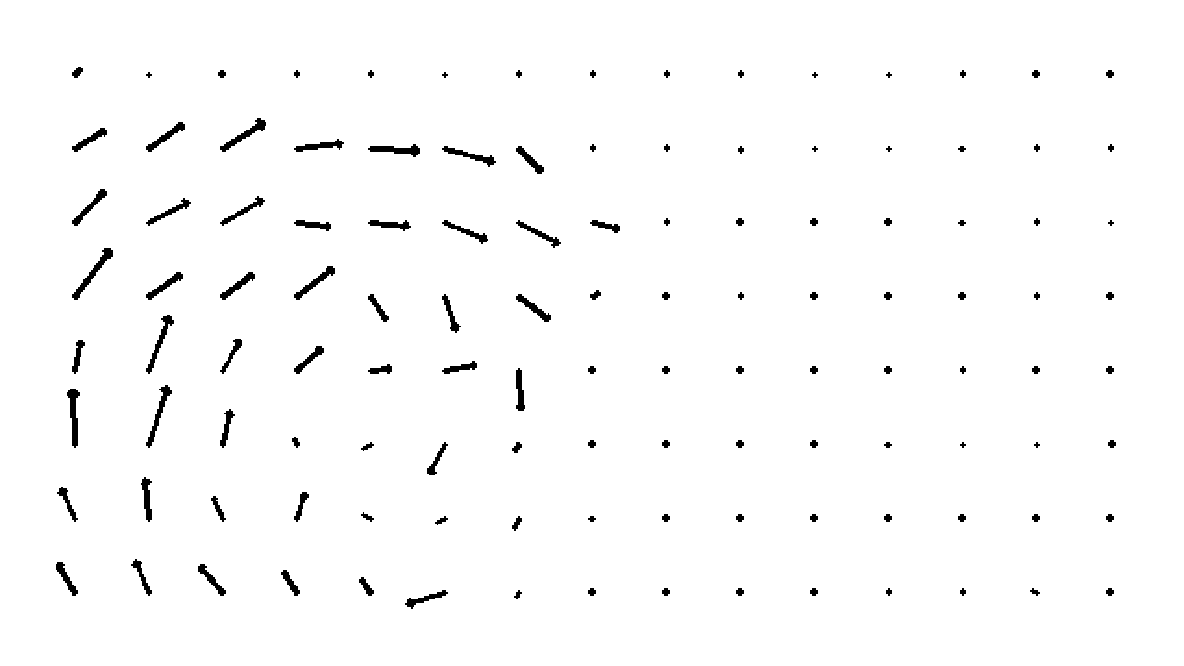
\includegraphics[width=11.2truecm, height=6.3truecm]{images/vectorField_screenshot.png}}
\caption{Képernyőfotó a vektormezőről, egy $8 \times 15$-ös rácsfelbontás mellett}
\label{fig:vectorfield}
\end{figure}

A kapott pontok párjaiból kiszámolhatjuk az elmozdulásvektorokat.

A mozgás detektálása rácspontok segítségével kevesebb számítást igényel, mintha minden pixel elmozdulását vizsgálnánk és az elmozdulás becslésére is elfogadható eredményeket kapunk.
A rács felbontását tetszőlegesen megadhatjuk. Minél nagyobb a felbontás, annál több pontot vizsgál a szoftver, ami nagyobb pontosságot is eredményez. Viszont a rácsfelbontás használata a futási időt is befolyásolja. Egy gyengébb hardver esetén nem ajánlott magas rácsfelbontás mellett futatnunk a programot, mivel tapasztalataim szerint jelentős lassulásra számíthatunk.

A rácspontok helyzetének meghatározásához elsősorban definiálnunk kell a rács felbontását és ismernünk kell a videófolyam felbontását is. Érdemes a képarány függvényében megválasztani a rács felbontásásnak értékeit. Pédául egy 16:9-es képarányú videófolyam esetén egy $9 \times 16$-es rács használata teljesen megfelelőnek tűnik, vagyis 9 sorban és 16 oszlopban lesznek elhelyezve a pontok az említett felbontás használata mellett. Ez 144 vizsgálandó pontot jelent.
A képtartomány széleit nem szükséges vizsgálnunk, hiszen a képből kilépő objektumok további helyzetét már nem tudjuk meghatározni és feltételezzük, hogy a lényeges mozgások nem a széleken történnek. Így érdemes egy bizonyos kereten belül elhelyeznünk a pontokat.

\bigskip

\noindent A következő algoritmus segítségével határozhatjuk meg a pontok helyzetét:

\medskip

\noindent \textbf{Rácspontok$\_$generálása}(@kép, @rács\_felbontás, @rács)\\
szélesség $\leftarrow$ kép.szélesség()\\
magasság $\leftarrow$  kép.magasság()\\
cella\_magasság $\leftarrow$ $\frac{\text{magasság}}{\text{rács\_felbontás}_0}$\\
cella\_szélesség $\leftarrow$ $\frac{\text{szélesség}}{\text{rács\_felbontás}_1}$\\
k $\leftarrow$ 0\\
\textbf{FOR} i $\leftarrow$ 0 \textbf{TO} $\text{rács\_felbontás}_0-1$ \textbf{DO}\\
\indent \textbf{FOR} j $\leftarrow$ 0 \textbf{TO} $\text{rács\_felbontás}_1-1$ \textbf{DO}\\
\indent \indent $\text{rács}_{k,0}$ $\leftarrow$ j $\times$ cella\_szélesség $+ \frac{\text{cella\_szélesség}}{2}$\\
\indent \indent $\text{rács}_{k,1}$ $\leftarrow$ i $\times$ cella\_magasság $+ \frac{\text{cella\_magasság}}{2}$\\
\indent \indent k $\leftarrow$ k + 1\\
\textbf{RETURN} rács

\Section{Hőtérkép}

A vektormező egyes pontjait vizsgálva szerkeszthetünk egy ún. \textit{Hőtérkép}-et, amelyben különböző intenzitásértékekkel jelöljük az egyes vektorok hosszait. Az általam definiált \textit{Hőtérkép} egy $n \times m$-es mátrix, ahol $n$ a vektormező sorainak, $m$ pedig az oszlopainak a száma. A \textit{Hőtérkép} minden eleme egy BGR (blue, green, red) hármas értékkel van ellátva. Ezen értékek jelölik az egyes elemek színét. A BGR színkódolás használata, a szokványos RGB helyett az \textit{OpenCV} egyik jellegzetessége.\\
Az értékek a következőképpen kerülnek kiszámításra:\\
\newline
\noindent \textbf{Hőtérkép$\_$kiszámítása}(@vektormező, érzékenység, @hőtérkép)\\ 
Input paraméter: vektormező (n$\times$m-es mátrix), érzékenység\\
Output paraméter: hőtérkép\\
\textbf{FOR} i $\leftarrow$ 1 \textbf{TO} Hossz(vektormező$_n$) \textbf{DO}\\
\indent \textbf{FOR} j $\leftarrow$ 1 \textbf{TO} Hossz(vektormező$_m$) \textbf{DO}\\
\indent \indent hőérték$_{ij}$ $\leftarrow$ hossz(vektormező$_{ij}$)*érzékenység\\
\indent \indent \textbf{IF} hőérték$_{ij}$ > 255\\
\indent \indent \indent \textbf{THEN} hőérték$_{ij}$ $\leftarrow$ 255\\
\indent \indent hőtérkép$_{ij}$ $\leftarrow$ (255-hőérték$_{ij}$, 0, hőérték$_{ij}$)\\
\textbf{RETURN} hőtérkép\\
\newline
0 pixel hosszúság esetén az adott indexű elem (255, 0, 0) értéket kap, vagyis kék színnel jelöljük. Ha egy adott vektor számított hőértéke eléri a 255-öt, a hozzá tartozó \textit{hőtérkép-érték} (0, 0, 255) intenzitásértéket kap, vagyis tiszta piros színnel fog megjelenni.
A \textit{érzékenység} értékkel állíthatjuk be, hogy mely vektorhosszakat vegyen a program figyelembe. Az érték megadja, hogy milyen mértékű legyen a vektorok nagyítása, befolyásolva ezzel a számított \textit{hőértéket}.
\begin{figure}[h]
\centering
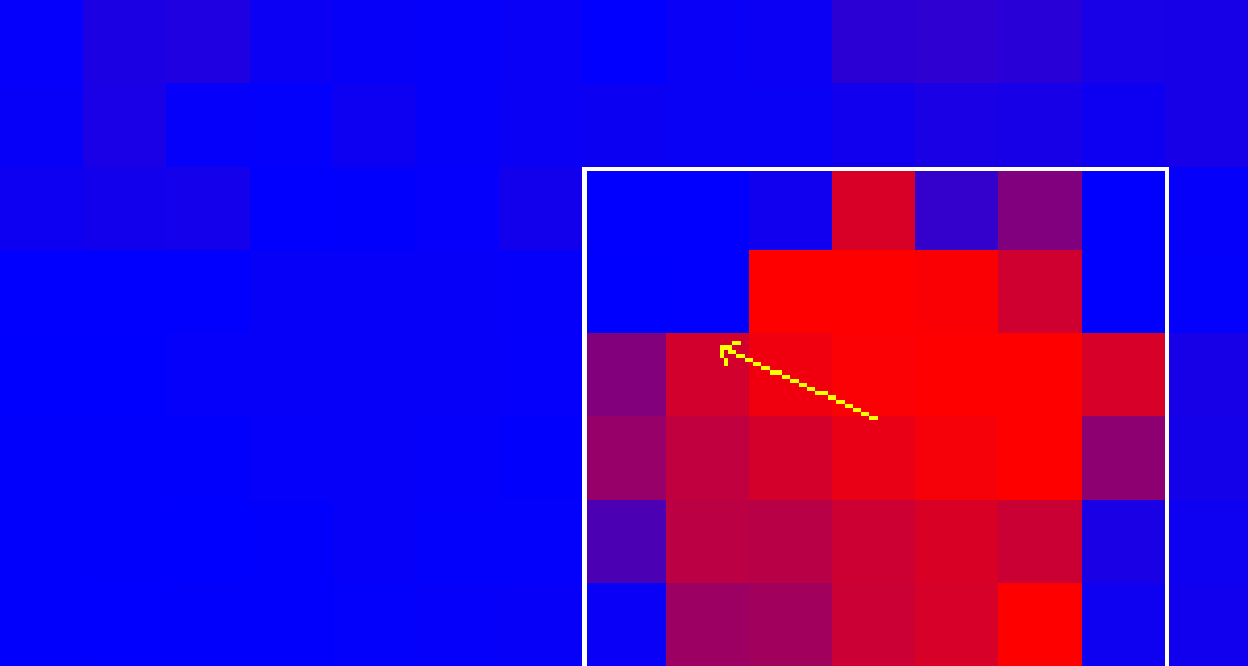
\includegraphics[width=11.2truecm, height=6.3truecm]{images/HeatMap_screenshot.png}
\caption{Képernyőfotó a hőtérképről}
\label{fig:heatmap}
\end{figure}
A három színcsatorna használata csupán megjelenítés szempontjából előnyös, mivel a kék és a piros szín elüt egymástól, így szabad szemmel nézve jobban meg tudjuk figyelni a kiszámított értékeket. Viszont a program számára a szürkeárnyalatos kép is elegendő információt hordoz, így a feldolgozás során a fent kikevert színértékeknek nincsen további jelentősége.

Az így kapott mátrixból ezután különféle információkat nyerhetünk ki. Az intenzitás értékeket vizsgálva meghatározhatjuk a nagyobb elmozdulások csoportjait. Ehhez küszöbölni kell a mátrixot, majd a kapott képen kontúrok keresésével meg lehet állapítani, hogy mely vektorok tartoznak egy csoportba. A csoportokat egy bizonyos intenzitás érték fölött érdemes keresni, vagyis az olyan vektorok összetartozó halmazai lehetnek érdekesek számunkra, amelyekben a vektorok hossza egy bizonyos határt elér. Az esetlegesen előforduló képzajok és az a videófolyamon megfigyelhető egyéb anomáliák miatt, amelyek a vektormező értékeire is hatással lehetnek, meg kell szabnunk a csoportok minimális területét. A megfelelően megválasztott értékek mellett a képzajból származó hibás értékek nem befolyásolják a program működését.
A \ref{fig:heatmap} ábrán megfigyelhető, hogy az összetartozó értékek fehér kerettel vannak jelölve. Továbbá a csoportok elmozdulásának irányai sárga nyilakkal vannak ábrázolva. A csoportokat külön-külön vizsgálva további értékes információkhoz juthatunk. Ilyen például az egyes csoportok iránya is, amelyet egy lokális eredővektor számításából kaphatunk meg. A csoportokat felhasználhatjuk további funkciók megvalósítására is, mint például a \textit{Többpontos kezelés}, a \textit{Rotation} és a \textit{Symbol}.

\Section{Gépi tanulásos módszerek, teljesítménymérések}

A dolgozatom programjához szükséges modellek betanításhoz felügyelt tanítási módszert kívánok alkalmazni, \textit{offline} adatkészletekkel. Az ilyen típusú tanító módszererek hátrányai közé sorolhatjuk a rugalmatlanságot is, vagyis az alkalmazóképesség hiányát is. Az \textit{online} tanulásos módszerek ezzel ellentétben sokkal jobban alkalmazkodnak, hiszen működés közben a valós világ éppen aktuális jellegzetességeihez igazítják magukat. Az \textit{online} módszerek előnye lehet a kisebb memória igény is, hiszen kevesebb adatmennyiség van jelen a futás során. Ez egyben a módszerek hátrányát is jelenti, mivel könnyen felejtenek az ilyen megoldások és a drasztikus, hirtelen változásokra rosszabbul reagálnak, mint az \textit{offline} módszerek. \cite{geron2019hands}

A tanítómintát két részre szokás bontani, tanító adatkészletre és teszt részre. A tanító adatkészletünk a modell tanítására szolgál, míg a teszt adatkészlet segítségével pedig a már betanított modellünk teljesítményét mérhetjük. A teszt adatkészlet elkülönítése azért szükséges, hogy betanítás után olyan adatokkal is tudjuk vizsgálni a modell teljesítményét, melyek nem egyeznek meg a tanítómintával. Így pontosabb eredményeket kaphatunk a teljesítményről, hiszen feltételezhetjük, hogy "élesben" is hasonlóan eredményeket fog szolgáltatni. Fontos a helyes arány megválasztása a felbontásnál, általánosan 70\% tanító és 30\% teszt adat javasolt. \cite{geron2019hands}

Az adatkészlet helyes mennyiségének meghatározása sok tényezőtől függhet, de belátható, hogy minél több adattal rendelkezünk az adott problémáról, annál kevésbé fognak érvényesülni az egyes osztályozó típusok előnyei. \cite{geron2019hands} Az adatok osztályok közti eloszlása is hatással lehet az osztályozó teljesítményére. Javasolt kiegyensúlyozott adatkészlettel dolgozni. Viszont az osztályozó hibáit bizonyos mértékig orvosolhatjuk az egyes osztályokon belül található adatok számának változtatásával. Az osztályozó teljesítményét tovább növelhetjük automatikus paraméterkereséssel, \textit{Grid-Search}-el is, amelyel az optimális paramétereket kívánjuk megtalálni. \cite{koesmarno2019class}

A program működése során felmerülő feladatokhoz a \textit{Random Forest} típusú osztályozót választottam, amely döntési fákat alkalmaz a részminták halmazán, majd átlagolás segítségével hozza meg a döntéseket. Az egyszerre több osztályozó segítségével történő osztályozást \textit{ensemble} \cite{geron2019hands}, vagyis együttes módszereknek nevezzük.

A betanított modell teljesítményének mérésére két módszert kívánok alkalmazni, a \textit{Cross-Validatiot} és a \textit{Confusion Matrix} ábrázolást.

\SubSection{Cross-Validation}

A \textit{$k$-hajtásos Cross-Validation} technika a mintát $k$ egyenlő részre osztja, majd egy ciklussal végigmegy a $k$-kon: a minta $k-1$ részével tanítja a modellt, majd a maradékon pedig ellenőrzi és kiértékeli az így beatanított modell teljesítményét. Így $k$ darab eredményt kapunk, melyet átlagából következtethetéseket vonhatunk le a modell teljesítményéről.

Például a \textit{Symbol}-hoz készített három osztállyal rendelkező 348 elemű adatkészletem 70\%-os (243 db) tanítómintájára, $k=5$ hajtással elvégzett \textit{Cross-Validation} teljesítménymérése a következő:
\begin{align*}
	k_1 &= 0.9388\\
	k_2 &= 0.9796\\
	k_3 &= 0.9592\\
	k_4 &= 0.9167\\
	k_5 &= 0.9792\\
	\bar{k} &= 0.9547
\end{align*}
Ahol $\bar{k}$ a minta átlaga.\\
Az eredményekhez érdemes hibát is számolni, majd segítségével konfidencia intervallumot megadni. Legyen például a konfidenciaintervallum 95\%-os és a hibát Standard hibaként tekintsük.
\begin{align*}
	\boldsymbol{CI}(95) = m (+/-) 1.96 \cdot \frac{s}{\sqrt[]{n}}
\end{align*}
Ahol $m$ a minta átlaga, $s$ a szórás, $n$ pedig a minta darabszáma.\\
Az eredmények alapján a betanított modellünk $95.47 (+/- 2.12)$\%-os pontossággal rendelkezik, vagyis ennyi valószínűséggel hoz helyes döntéseket. Hogy megvizsgáljuk, hogy mely esetekben téved a modellünk egy másik teljesítménymérő módszer segítségére lesz szükségünk, a \textit{Confusion Matrix} ábrázolásra.

\SubSection{Confusion Matrix}

\begin{figure}[h]
\centering
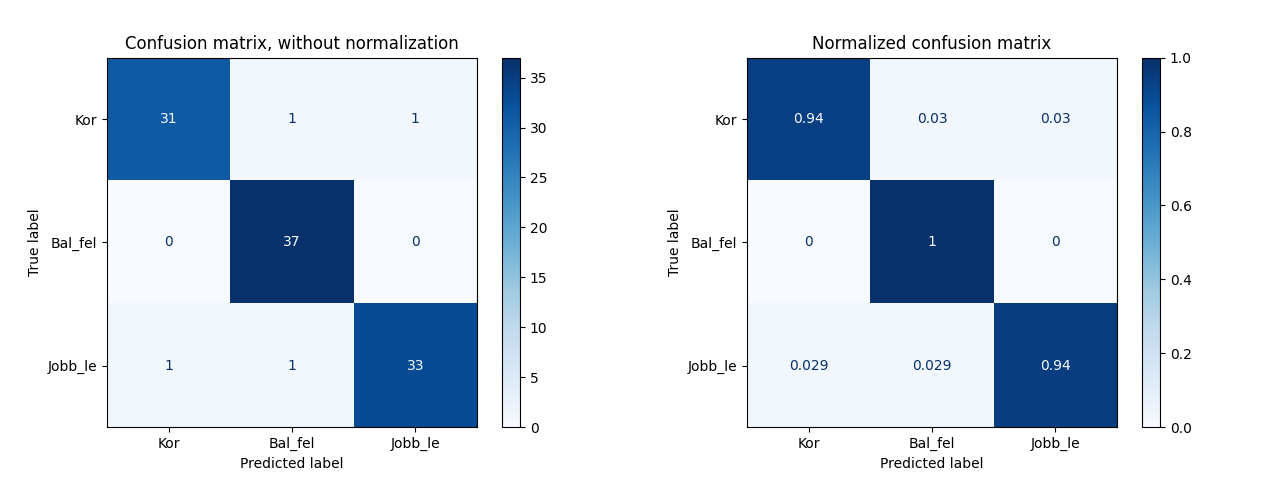
\includegraphics[width=\textwidth]{images/confusion_m.png}
\caption{\textit{Confusion Matrix}-ok a \textit{Symbol} adatkészletre}
\label{fig:confusionm}
\end{figure}

A teljesítménymérésnek egy másik módja lehet az úgynevezett \textit{Confusion Matrix} módszer. Segítségével meg lehet figyelni a helyes és hibás döntések eloszlását egy mátrix formájában.\cite{koesmarno2019class}
A már betanított modellünket a teszt adatkészlettel ellenőriztetjük, majd az eredmények alapján megszerkeszthetjük a mátrixunkat. Két fajta eredmény keletkezhet minden osztályban: Helyes becslés és hibás becslés. Mátrix soraiban az adatkészletben szerepő osztályok találhatók, míg oszlopaiban a becslések. Az általános \textit{Confusion Matrix} főátlójában a helyes becslések eloszlása figyelhető meg. Az átló alatti és feletti részeken pedig a hibás becslések, vagyis a hibás reosztályozások számai. A mátrixból jól leolvasható, hogy mely osztályokat kever össze az adott modell. A normalizált mátrix csupán arra szolgál, hogy nagy mennyiségű adatok mellett is jól kiolvashatóak legyenek az egyes osztályokra hozott becslések mértékei.
A \ref{fig:confusionm} ábrán megfigyelhető a \textit{Symbol} adatkészletre betanított modell, teszt mintahalmazzal való ellenőrzése \textit{Confusion Matrix} ábrázolással. Megfigyelhető, hogy milyen esetekben hozott hibás döntést a modellünk.

\Section{Kontrollpontok és vektorok számítása}

\SubSection{Sweep}

A \textit{Sweep} gesztus két tulajdonsággal írható le: A mozgás irányával és hosszával. A mozgás irányát egy $\vec{v}\in\mathbb{R^2}$ irányvektorral határozhatunk meg, amelyet a \textit{vektormező} globális eredővektoraként kapunk meg.
\begin{align*}
  \vec{v} = \sum_{i=1}^n\vec{u_i}
\end{align*}
, ahol $\vec{u}$ a teljes képre vett vektormező vektorai.\\
A mozgás hossza a vektormező vektorainak átlagos hosszában mérhető és pixelszámban fejezhető ki.
\begin{figure}[h]
\centering
\frame{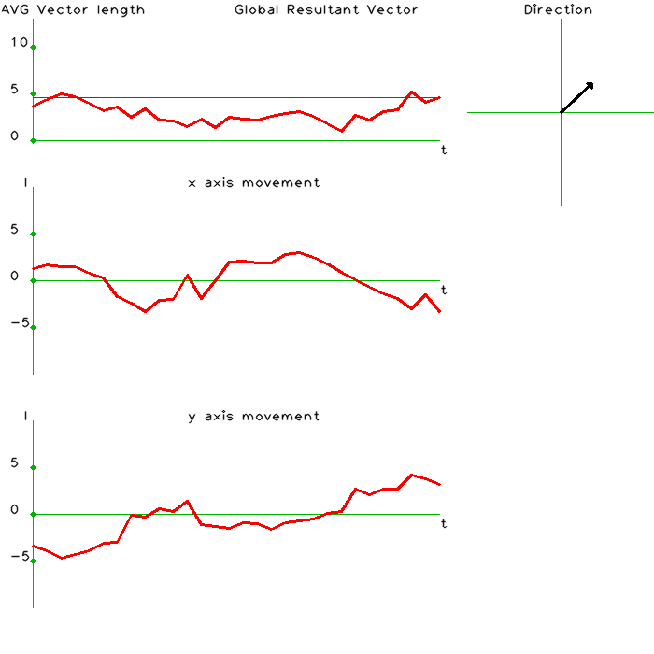
\includegraphics[width=8.0truecm]{images/ResultantPlot_screenshot.png}}
\caption{Képernyőfotó a globális eredővektor grafikonjáról}
\label{fig:resultantplot}
\end{figure}

Az ábrán megfigyelhető a globális eredő vektor hosszainak változása egy 30 képkockás \textit{csúszóablakban} és az éppen aktuális irányvektor is, valamint az $x$ és $y$ tengelyen megfigyelhető mozgások változásai is.

\SubSection{Shift}

A \textit{Shift} tulajdonsággal rendelkező virtuális elemeknek mindig van egy aktuális pozíciójuk $(x,y)$, szélességük és magasságuk $(w,h)$, illetve sebességértékük $v_{xy}$ (a két tengelyre vonatkozóan). A pozíciót a virtuális elem bal felső sarkának tekintsük.

A \textit{Shift} viselkedésének meghatározásához első lépésként az adott virtuális elem területére eső vektorokból $\vec{v}_l$  lokális irányvektort számolunk. Az elem területére eső vektorok meghatározható az elem pozíciója és a mérete alapján a következő módon:

Jelöljük $\boldsymbol P \in \mathbb{R}^2$-vel a virtuális elem pozícióját $(x,y)$, $\boldsymbol D \in \mathbb{R}^2$-vel pedig a dimenzióját (szélesség, magasság).
A rácspontok alapján kiszámolhatjuk a lépésközt is, ami rács első koordinátájának az összege lesz. Ezt jelöljük $\boldsymbol L \in \mathbb{R}$-el. 
\begin{align*}
	\boldsymbol L = \textit{rács}_{0,0} + \textit{rács}_{0,1}
\end{align*}
Ha rácsot háromdimenziós vektornak tekintjük, vagyis egy $n\times m$-es mátrixnak, ahol $n$ a rács sorait, $m$ pedig az oszlopait jelöli.\\
A részmátrix kezdőpozícióját jelöljük $\boldsymbol {RM}poz \in \mathbb{R}^2$-vel,\\
dimenzióját pedig $\boldsymbol {RM}dim \in \mathbb{R}^2$-vel.
\begin{align*}
	\boldsymbol {RM}poz &= \left\lfloor \frac{\boldsymbol P}{\boldsymbol L} \right\rfloor\\
	\boldsymbol {RM}dim &= \left\lfloor \frac{\boldsymbol D}{\boldsymbol L} \right\rfloor
\end{align*}
Jelöljük $\vec{u}$-val a vektormező irányvektorait.
\begin{align*}
  \vec{v_l} &= \frac{\sum_{i=\boldsymbol {RM}poz_1}^{\boldsymbol {RM}dim_1} \sum_{j=\boldsymbol {RM}poz_0}^{\boldsymbol {RM}dim_0} \vec{u}_{ij}}{\boldsymbol {RM}dim_0 \cdot \boldsymbol {RM}dim_1}
\end{align*}
Így megkaptuk a $\vec{v_l}$ lokális irányvektort, amely egyben az elem elmozdulásvektora is. Segítségével kiszámolhatjuk az elem sebességét:
\begin{align*}
  v_{xy} = v_{xy} + \frac{\vec{v}_l}{\boldsymbol {RM}dim_0 \cdot \boldsymbol {RM}dim_1} \cdot \textit{gyorsulás}
\end{align*}
, ahol $\textit{gyorsulás} > 0$.\\
Az elem pozíciója ($\boldsymbol P$) a sebesség függvényében változik.
\begin{align*}
  \boldsymbol P = \boldsymbol P+v_{xy}
\end{align*}
A sebesség értéket minden iteráció végén tompítani kell, hogy a kezelt virtuális elem meg tudjon állni egy bizonyos ponton. Ha az adott elemet nem éri tovább erő, akkor a tompítás lassulást eredményez, a sebesség csökkenni fog. Olyan hatást is el tudunk érni egy helyesen megválasztott értékkel, mintha az eltolás után az elem csúszós felületen mozogna és így fokozatosan lassul le az iterációk során.
\begin{align*}
  v_{xy} = v_{xy} \cdot \textit{tompítás}
\end{align*}
, ahol $0 \leq \textit{tompítás} < 1$

\SubSection{Blink}

A \textit{Blink} gesztusok felismerésére elsősorban egy ún. \textit{Frame differencing} technikát kell alkalmaznunk.
Ehhez a videófolyam aktuális képkockájának és az eggyel korábbi képkockájának abszolút különbségét kell meghatározni, majd az így kapott képen küszöbölést kell végrehajtani. Eredményképp egy olyan képet kapunk, amelyen az elmozdulás figyelhető meg fehér színnel jelölve. A keletkezett képen különféle alakzatok alakulhatnak ki. Az egyes mozdulatok hasonló nyomot hagynak maguk után. Így tehát egy \textit{Blink} mozdulat leadásakor jellegzetes mintázat rajzolódik ki.

\begin{figure}[h]
\centering

\includegraphics[width=4truecm, height=4truecm]{images/Grab_screenshot.png}
\caption{Egy Blink mozdulat pillanatképe}
\label{fig:blink}
\end{figure}

A \textit{Frame differencing} technika a teljes képtartományra vonatkozik, minden iterációban elvégezhetjük, hogy a videfolyamon történő mozgásról információkat kapjunk. A \ref{fig:blink} ábrán megfigyelhető, hogy nem csupán a legfrissebb két képkocka adatai vannak jelen a képen. Ezt a jelenséget egy keverési technikával érhetjük el. A korábbi mozdulatok rajzolatai alacsonyabb intenzitás értékekkel jelennek meg, míg a legfrissebb értékek 255 intenzitással vannak jelölve.

A gesztus detektálásához rögzített hosszúságú jellegvektorokra lesz szükségünk. A \textit{Frame differencing} technika képének dimenzió megegyeznek a videófolyam felbontásával. Így például $640\times480$ felbontás mellett 307200 hosszúságú jellegvektorokat kapunk. A gesztus ily módon történő detektálása nem a legoptimálisabb megoldás. A \textit{Frame differencing} kép felbontásának csökkentésével pedig romolhat az információ minősége is.

A \textit{Blink} gesztusról feltételezhetjük, hogy a videófolyam egy kis területén fog jelentkezni. A terület meghatározásához segítségül kell hívnunk a \textit{Hőtérkép} által meghatározott csoportokat. A gesztus kiadásának pillanatában feltételezhetjük, hogy a \textit{Blink}-en kívül más egyéb mozgás nem figyelhető meg a videófolyamon, amely a \textit{Hőtérkép} számításánal újabb csoportokat jelentene. Így tehát a \textit{Blink} további vizsgálatának előfeltétele, hogy a \textit{Hőtérképen} csupán egyetlen összefüggő csoport helyezkedjen el.
\begin{figure}[h]
\centering
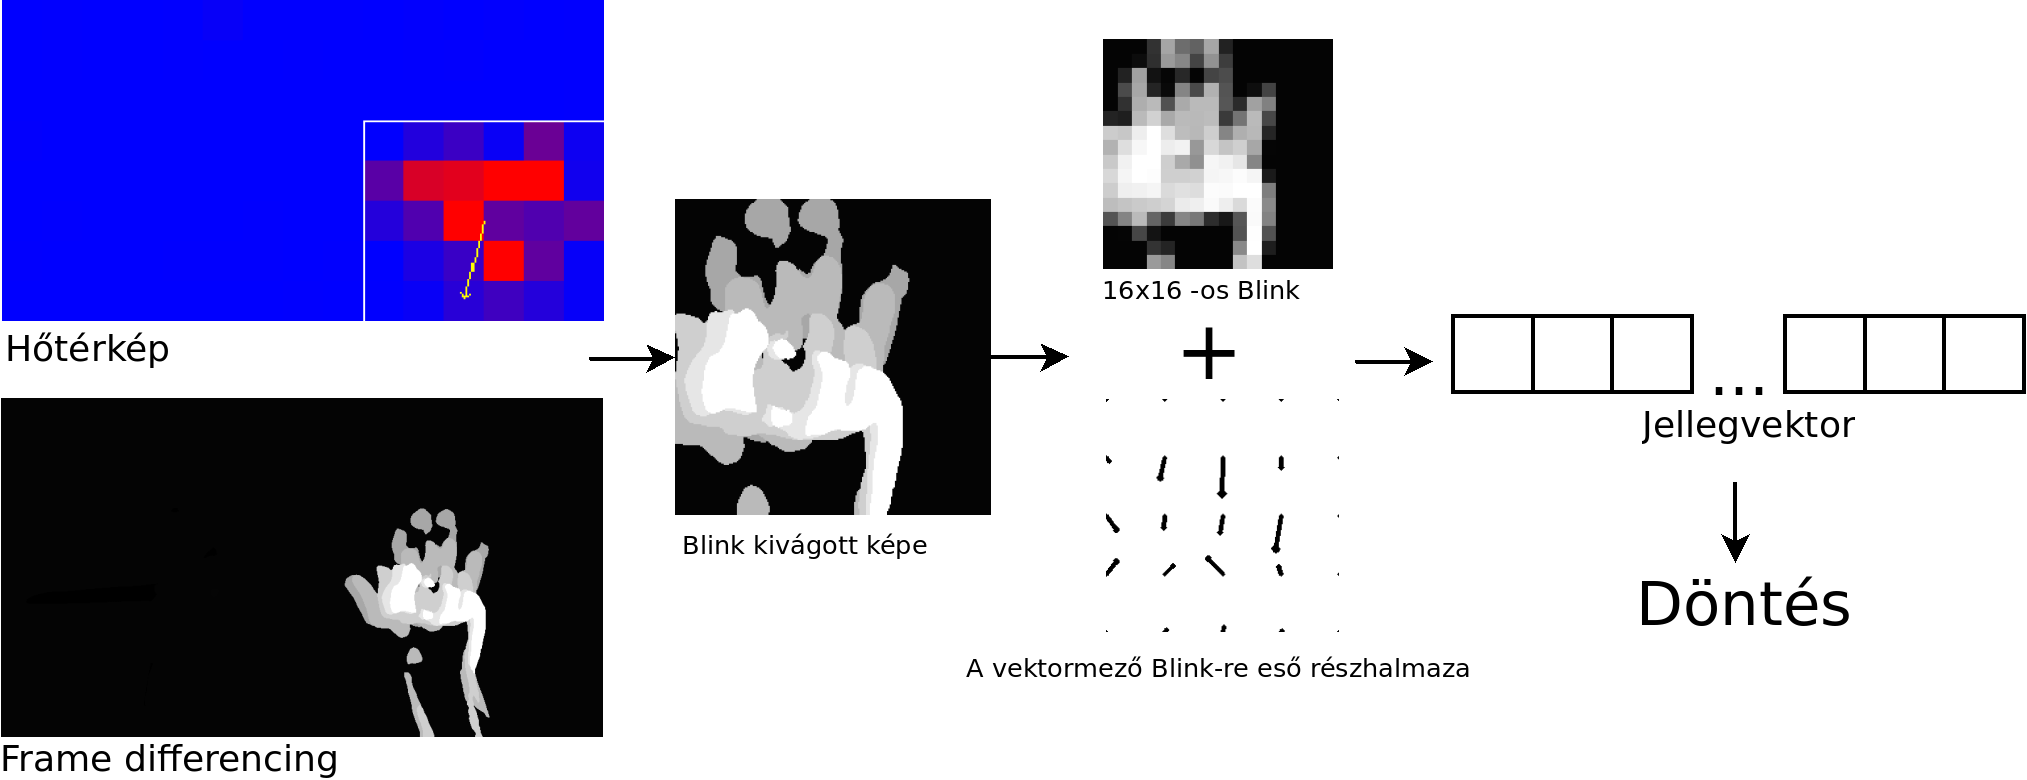
\includegraphics[width=\textwidth]{images/blink_flow.png}
\caption{A gesztus detektálásának folyamata}
\label{fig:blinkflow}
\end{figure}

A csoport változásait ezután figyelemmel kísérjük, a tulajdonságait egy szűrési feltétel után rögzítjük. Mivel a \textit{Blink} gesztus várhatóan a vektormező egy viszonylag kis területen figyelhető meg, ezért egy bizonyos \textit{Hőtérkép-csoport} méret fölött nem érdemes további vizsgálatokat végrehajtani. Ha a \textit{Hőtérképen} megfigyelhető csoport területe meghaladja a 25 pixelt, akkor arról a csoportról feltételezhetjük, hogy nem tartalmaz \textit{Blink} gesztust. Természetesen ez a mennyiség rácsfelbontásokként változhat. Egy nagy sűrűségű rácson valószínűleg már alacsony lenne ez az érték, viszont az ajánlott rácsfelbontás mellett jól működik. Mint korábban kifejtettem, nem érdemes túl sűrű rácsot alkalmazni, így a területre megszabott korlát az indokolt rácsfelbontásokig megfelelőnek tűnik.

Ha a területre vonatkozó szűrés eredményes lesz, meghatározhatjuk a \textit{Blink} gesztus középpontját. A szűrésen átesett csoport nem minden esetben négyzetes. A rögzített jellegvektor hossz szükségessége miatt minden esetben egy $5\times5$-ös részmátrixot kell meghatároznunk a \textit{Vektormezőre} nézven. A részmátrix középpontját a \textit{Hőtérképből} kinyert csoport középpontja adja. A mátrix szélein és a sarkoknál, az indexelés helyessége miatt meg kell szabnunk, hogy a középpont minimum 2 lépés távolságra lehet a szélektől. Ha esetleg ez nem teljesülne, a legközelebbi helyes pontot jelöljük ki a \textit{Blink} gesztus középpontjának. A részmátrix segítségével meghatározhatjuk a \textit{Vektormező} $5\times5$-ös csoportra eső irányvektorait is. A gesztus területére eső irányvektorokat a pontosabb becslés érdekében használjuk majd fel.

Ha sikeresen meghatároztuk a \textit{Blink}-re eső \textit{vektorokat} és azok indexeit a \textit{Vektormezőn} belül, később a \textit{Rács} indexelt pontjainak értékeit felhasználva kiemelhetjük a \textit{Frame differencing} képből a \textit{Blink} gesztus tartományát. Az eredeti képből kivágott kép jóval kisebb lesz, a felesleges értékekből is kevesebb jelentkezik majd. A \ref{fig:blink} ábrán megfigyelhető egy, a program által kivágott \textit{Blink} képe, amin jó látható, hogy a felesleges értékek nagy részétől sikeresen megszabadultunk.

Az előbbi feldolgozási folyamat végrehajtását is egy további feltételhez kell kötnünk, ez pedig legyen a \textit{Hőtérképen} megfigyelhető csoportok teljes hiánya, vagyis az a pillanat, amikor a \textit{Blink} gesztus befejeződik. Természetesen egy további feltétel az is, hogy létezzen bejegyzés a lehetséges \textit{Blink} gesztus tulajdonságaira is. A korábban meghatározott középpont és indexek alapján ilyenkor kivágjuk a \textit{Frame differencing} eljárással kapott képből a feltételezett \textit{Blink} gesztus képét.

A kapott kép dimenzióit skálázással tovább csökkenthetjük egy bizonyos pontig, hogy a detektálás minél kevesebb memóriát vegyen igénybe. Szintén empirikus értékek szerint a gesztus képét egy $16\times16$-os mátrixra csökkenthetjük. Ebben az esetben a jellegvektorok hossza 256-ra csökken. Mint említettem, a vektormező értékeit is felhasználhatjuk a pontosabb detektálás érdekében. Érdemes irányvektorokat használni, így a gesztus a videófolyamon megfigyelhető helyzete nem befolyásolja a végeredményt. Mivel $5\times5$-ös területet szabtunk meg, ez további $2\cdot 25$ darab jellegvektort jelent.
\begin{figure}[h]
\centering
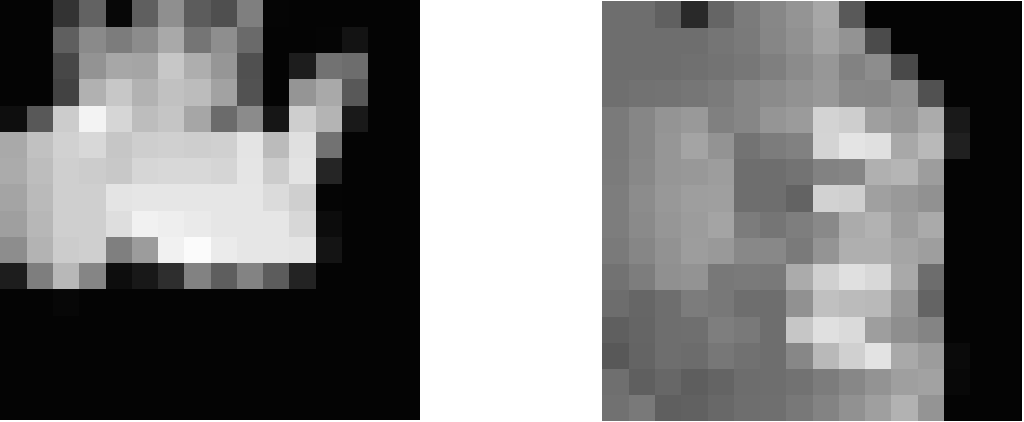
\includegraphics[width=7.00truecm]{images/blink-not_blink.png}
\caption{Egy \textit{Blink} és egy teljesen más gesztus képe ($16\times16$-os felbontással)}
\label{fig:blinkvsnotblink}
\end{figure}

Amint rendelkezésünkre állnak a kapott adatok, jellegvektort formálhatunk belőlük a következő módon: A $16\times16$ felbontású képet kinyújtjuk és az irányvektorok csoportjaival is hasonlóképpen járunk el. A kapott listákat pedig konkatenáljuk, vagyis egymás után fűzzük őket. Így egy 306 hosszúságú jellegvektort kapunk, melyben benne vannak a kép intenzitásértékei és a mozdulatot leíró részvektortér adatai is. A jellegvektor segítségével ezután a betanított modellünk osztályozza a gesztust.

A \textit{Blink} detektálásához egy bináris osztályozóra lesz szükségünk. A bináris osztályozók két osztályt ismernek, esetünkben az igaz érték jelenti majd a \textit{Blink} gesztust, a hamis érték pedig az olyan gesztusokat, amelyek nagy valószínűséggel nem \textit{Blink}-ek. A modell betanításához egy sor \textit{Blink}-et kellett rögzítenem, a hamis osztály adatainak gyűjtésénél pedig elindítottam a programot és próbáltam olyan mozdulatokat végrehajtani a kamera előtt, melyeket egy prezentáció alkalmával a prezentáló személy is leadna. Ilyenek a magyarázó mozgás, a mutogatás, gesztikulálás. Egy \textit{Blink} és egy másik mozdulat képei a \ref{fig:blinkvsnotblink} ábrán figyelhetők meg. Amint rendelkezésre állt a kívánt adatmennyiség, a rögzítést leállítottam és a kapott adatkészlettel betanítottam az osztályozó modellt.
\begin{figure}[h]
\centering
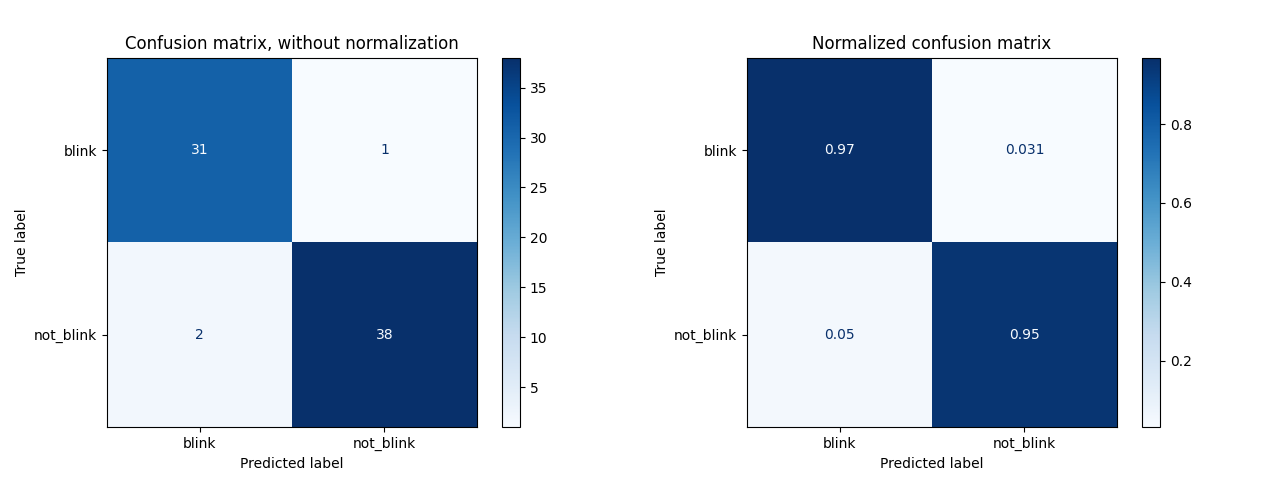
\includegraphics[width=\textwidth]{images/blink_confusion.png}
\caption{\textit{Confusion Matrix}-ok a \textit{Blink} adatkészletre}
\label{fig:blinkconfusion}
\end{figure}

A \textit{Blink} gesztus képe természetesen más módszerekkel is meghatározható, egy egyszerűbb megközelítése lehet a problémának a \textit{blob} alapű szűrés elvégzése. A \textit{blob} közös tulajdonság(okkal) rendelkező összefüggő pixelhalmaz. A közös tulajdonságok közé tartozhatnak a konvexitás, méret, alak, intenzitás-értékek, stb\ldots A \textit{Frame differencing} eljárás során keletkezett képen szabad szemmel is megfigyelhető, hogy az egyes \textit{Blink} gesztusok hol helyezkednek el, hiszen korábban megállapítottuk, hogy a kapott képen hasonló nyomot hagynak. Így a megfelelő paraméterekkel ellátott \textit{Blob detektor} segítségével meg lehetne határozni a \textit{Frame differencing} képén elhelyezkedő \textit{Blink} képeit. Ezen megoldás kétségkívül egyszerűbb megoldást jelentene, mint az általam használt eljárás, viszont a megfelelő paraméterek megválasztása időigényes feladat lehet. Az \textit{OpenCV}-ben található implementációt a \texttt{cv2.SimpleBlobDetector()} függvényben találhatjuk meg.

\SubSection{Drag and Drop}

A \textit{Drag} az elem elkapása utáni állapot jelenti, amikor a felhasználó az elkapott elem helyzetét szabadon változtathatja, majd új pozíciójára teheti (\textit{Drop}). Ennek a funkciónak a megvalósításához többféleképpen is hozzáláthatunk.

Az első ötletem szerint a vektormező vektorait felhasználva lokális eredővektor segítségével becsülte volna meg a program a mozgatandó virtuális elem új helyzetét. Ez a megoldás gyakorlatban az elvárásokat nem elégítette ki. Több probléma is adódott. A \textit{Rács} lyukacsossága miatt nem mindig esett vizsgálandó pont a mozgás helyére. Az egyes kiugró értékek is befolyásolták a végeredményt, a mozgatandó elemek ilyen esetekben gyorsabban mozogtak a vártnál. Ez a megoldás tehát nem tűnt stabilnak, a vektormező rácsának sűrítésével pedig a program jelentős lassulásba ütközött volna. Más megoldás után kellett kutatni.

Mivel a \textit{Drag and Drop}-ot előreláthatólag a prezentáló csak rövid időszakaszokban fogja használni, ezért a következő ötlettel áltam elő: a \textit{Blink} gesztus pozíciójára kontollpont(okat) illeszthetnénk, melyekre külön-külön elvégezhetnénk az \textit{Optical Flow} eljárást és a pont vagy a pontok súlypontjának pozíciója függvényében változna a mozgatandó virtuális elem pozíciója is. Már egyetlen kontrollpont használata is kielégítő eredményt adott. Több kontrollpont használata csupán csak a biztonság érdekében tűnik megfelelőnek. Ha esetleg egy pont új pozícióját rosszul becsülné meg az eljárás és a pont egy bizonyos ponton leragadna, akkor maradjanak olyan "tartalék" pontok is, amelyek biztosítanák a funkció helyes működését.

A követendő pont(ok) helyes megválasztásánál figyelembe vehetjük a \textit{Blink} képét. A képen megyfigyelhető legnagyobb intenzitásértékű pontok koordinátájának a súlypontját meghatározhatjuk, hogy az elhelyezendő pont a lehető legnagyobb valószínűséggel a prezentáló személy \textit{Blink} gesztust végrehajtó kézfejére essen. Viszont a \textit{Blink} gesztus kiszámolt középpontját is felhasználhatjuk erre a célra, hiszen már az is megfelelő pontosságot biztosít.

\SubSection{Rotation}

A \textit{Rotation} gesztus két tulajdonsággal íható le: ezen gesztusnak mindig létezik egy elméleti középpontja, ami körül történik az elmozdulás, valamint van iránya is.
Becslést adni a mozgás lehetséges középpontjának pozíciójára a vektormező elemzésével célszerű.
A vektorokhoz egyenes egyenleteket szerkeszthetünk. Az egyenes egyenletének egy pontja a vektor kezdőpontja lesz, a normálvektora pedig az egyenes irányvektora.

\begin{figure}[h]
\centering
\frame{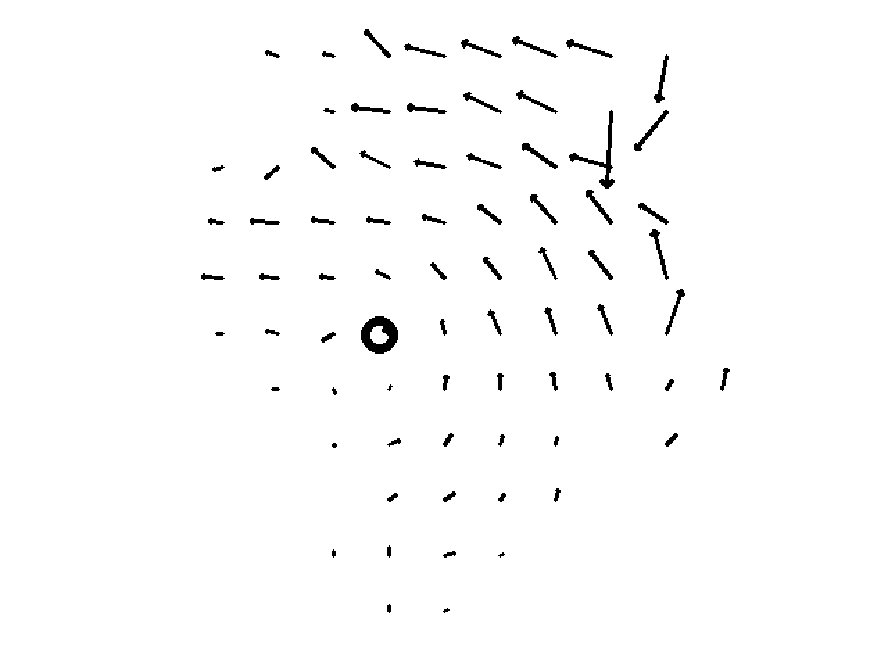
\includegraphics[width=8.88truecm, height=6.66truecm]{images/swirl_screenshot.png}}
\caption{A vektormező egy állapota a becsült forgási középponttal}
\label{fig:rotation}
\end{figure}

Két egyenletből álló egyenletrenszer megoldásaként megkapjuk az $x,y$ ismeretlen értékeket, melyek a két egyenes metszéspontjának a pozícióját adják meg.
A metszéspontokat számolva létrejön egy ponthalmaz, amelynek súlypontja az elméleti középpont közelében fog elhelyezkedni. A futásidő csökkentése érdekében érdemes csupán csak a szomszédos vektorok egyenleteit megoldani. A becslés pontossága viszont így romlani fog.
Ha pedig több \textit{Rotation} pontot is vizsgálni szeretnénk, akkor segítségül hívhatjuk a \textit{Hőtérkép}-ből kinyert vektorcsoportok halmazait, majd ezen csoportokon külön-külön elvégezhetjük az eljárást a lokális súlypontok után kutatva.

Az irány meghatározásához számolhatunk forgási szöget is. Ezt legegyszerűbben az \textit{arctg2} függgvénnyel tehetjük meg, amely segítségével a síkvektorok $y$ és $x$ koordinátáiból meghatározhatjuk az $x$-tengellyel bezárt szögüket.
\begin{align*}
		\text{arctg2$(y,x)$} =
  			\begin{cases}
    			\text{arctg$\left(\frac{y}{x}\right)$} & \text{, ha $x\geq \vert y \vert$,} \\
    			\frac{\pi}{2}-\text{arctg$\left(\frac{x}{y}\right)$} & \text{, ha $y\geq \vert x \vert$,}\\
    			-\frac{\pi}{2}-\text{arctg$\left(\frac{x}{y}\right)$} & \text{, ha $y\leq -\vert x \vert$,}\\
    			\pi+\text{arctg$\left(\frac{y}{x}\right)$} & \text{, ha $x \leq -y \leq 0$,}\\
    			-\pi+\text{arctg$\left(\frac{y}{x}\right)$} & \text{, ha $x \leq y \leq 0$}\\
  			\end{cases}
\end{align*}
% forrás? Wiki
A vizsgált vektorokra elvégézhetjük az \textit{arctg2}-t, majd átlagot vonva a kapott értékekből egy átlagos forgási szöget kapunk.

\SubSection{Többpontos kezelés}

A \textit{Hőtérkép}-et vizsgálva azonosíthatunk és elkülöníthetünk vektorok halmazait egymástól. Az így kapott csoportokat vizsgálva további funkciókat valósíthatunk meg. A több ponttal irányítható funkciók közé tartozhatnak a \textit{Widget}-eken végrehajtható különféle manipulációk, mint például a skálázás is. További komplexebb gesztusok felismeréséhez is felhasználhatnánk a pontok egymáshoz képesti vizsgálatából kapott eredményeket.
Minden vektorcsoporthoz tartozik egy-egy lokális eredővektorból számított irányvektor, mely a vektorcsoport elmozdulásának irányát mutatja.
A skálázás műveletéhez két vektorcsoportot feltételezve az alábbi módon vizsgálhatjuk a két pont egymáshoz képesti elmozdulását.
Irányok esetében $\vec{u},\vec{v}\in \mathbb{R^2}$ esetén
\begin{align*}
\vmatrix \vec{u}+\vec{v} \endvmatrix &< \varepsilon_{\text{irány}}\\
&\approx \vec{0}
\end{align*}
Amennyiben a két pont iránya teljesen ellentétes, akkor a kapott érték a null vektorhoz közelít. Érdemes normalizált vektorokat használni, ha csupán az elmozdulás irányát szeretnénk vizsgálni és az egyes lokális irányvektorok hosszától el szeretnénk tekinteni.

\SubSection{Symbol}

A prezentáló személy bizonyos mozdulatokat elvégezve további funkciókat érhet el. Az ilyen gesztusok egy fajtája általában a magyarázó mozgástól eltérőek, bizonyos pályákat követnek. Ilyen mozdulatok lehetnek például egy kör, vagy egy L betű, vagy különféle minták rajzolása levegőbe. Az egyes mozdulatok hasonló mintázatot követnek.

A dolgozat programjához mellékelt \textit{Symbol} adatkészlet három gesztus adatait tartalmazza. A három mozdulat a következő neveket kapta:
\begin{itemize}
	\item \textit{Gamma}
	\item \textit{Omikron}
	\item \textit{BRC} (Bottom Right Corner, vagyis jobb alsó sarok - az Unicode (U+231F) karakternek felel meg)
\end{itemize}
\begin{figure}[h]
\centering
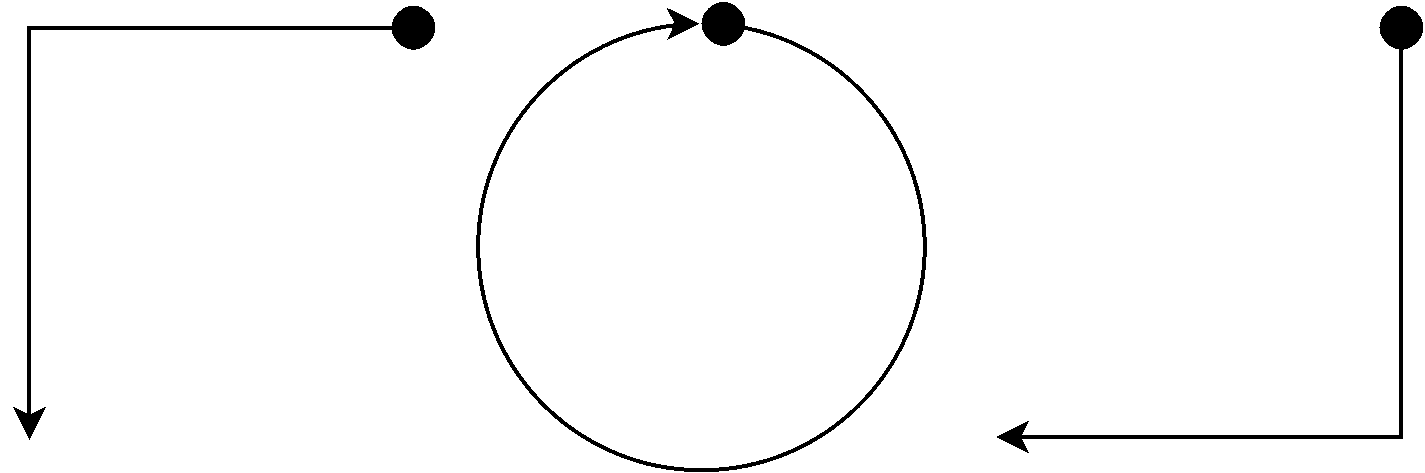
\includegraphics[width=10truecm]{images/symbols.png}
\caption{\textit{Gamma}, \textit{Omikron}, \textit{BRC}}
\label{fig:symbols}
\end{figure}

Ezen gesztusokra betanított osztályozó modell \textit{Confusion Matrix}-a a \ref{fig:confusionm} ábrán figyelhető meg. Belátható, hogy az osztályozó modell pontossága a minták között megfigyelhető viszonylag nagy távolságoknak is köszönhető.

Az ilyen típusú gesztusok felismeréséhez felhasználhatjuk az \textit{OCR}, vagyis az \textit{Optical Character recognition} (Optikai karakter felismerés) módszert is, mely írott karakterek felismerésére szolgál. 
Az OCR kipróbálásához rendelkezésre áll egy ingyenes adatkészlet is, a MNIST, amely 70.000 kisfelbontású képet tartalmaz írott számokról 0-9-ig. Segítségével különféle osztályozók taníthatók be, illetve az osztáyozók tejesítményének egyik mérőeszközévé vált az idők során. Az osztályozómodell betanításához a jellegvektorok értékeit a szürkeárnyalatos képek intenzitásértékei adják. Ha egy új osztályozó rendszert fejlesztenek, valószínűleg a MNIST adatkészlettel is kipróbálják azt. \cite{geron2019hands}

Mivel a probléma hasonlít az OCR-hez, hasonló megoldást alkalmazhatunk a levegőben leírt gesztusok felismeréséhez is. A mozdulat képét egy, a \textit{Hőtérképpel} megegyező méretű vászonra rögzíti a program. A vászon alapszíne fehér, vagyis 255 intenzitás értékekkel van ellátva. A gesztus képét a \textit{Hőtérkép} elemzésénel kinyert kontrollpontok rajzolják a vászonra: A vektorcsoportnak meghatározandó a súlypontja, mely a virtuális ecset hegyét jelenti. A súlypont elmozdulását a vásznon 0 intenzitásértékek követik, vagyis az elvégzett mozdulatok képei fekete színnel jelennek meg a vásznon. Mivel az egyes mozdulatok hasonló mintázatot követnek, a vásznon megjelenő képük is hasonló lesz.

\begin{figure}[h]
\centering
\frame{
\includegraphics[width=10truecm, height=7.33truecm]{images/OCR-Gesture.png}}
\caption{Egy levegőbe leírt \textit{Omikron} mintázata egy 11$\times$15-ös vásznon}
\label{fig:ocr-gesture}
\end{figure}

A vászon frissítése két módszerrel történik. Az elmozdulás értékek egy csúszóablakban helyezkednek el, amelyben maximum  30 érték kaphat helyet. Továbbá ha a \textit{Hőtérkép}-en nem figyelhető meg kontrollpont, az elmozdulás értékek törlése felgyorsul, míg a teljesen üres vásznot nem kapjuk.

A felismerés pillanatát feltételekhez kell kötnünk. A mozdulat rajzolatának végső formája akkor alakul ki, amikor a felhasználó befejezte az adott mozdulatot. Ilyen esetben a videófolyamon nem figyelhető meg további mozgás. Az időzítés egyik feltétele mindenképpen a mozgás hiányának kell lennie. Ez többféleképpen is megfigyelhető, vizsgálhatjuk a globális eredővektorunkat is, vagy a \textit{Hőtérkép} segítségével meghatározott csoportok számát is figyelembe vehetjük. Mivel a mintázat rajzolásához is a vektorok összetartozó csoportját használtuk fel, az időzítés egyik feltételének a vektorcsoportok hiányát szabhatjuk meg. Egy másik feltétel a rajzolat aktuális állapotára vonatkozhat. Figyelembe vehetjük a vonalhosszat is, vagyis egy bizonyos vonalhossz alatt nem végeznénk el az osztályozási becslést. Ezen két feltétel biztosítja, hogy az osztályozási művelet végrehajtása a megfelelő pillanatban történjen, elkerülve a felesleges számításokat, hibás becsléseket.

Mielőtt a gesztust reprezentáló képről döntene a modellünk, egy előfeldolgozási lépést kell végrehajtanunk rajta. A gesztus képe nem fogja betölteni a teljes vásznat, így sok felesleges értéket fog tartalmazni. Ennek kiküszöbölésére ki kell vágnunk a gesztus rajzolt képét és egy előre meghatározott felbontásra kell konvertálnunk. Tapasztalati alapokon a 11 $\times$ 15 -ös felbontás megfelelőnek tűnik, így minden egyes kivágott képet ilyen felbontásra kell alakítanunk. Ezen előfeldolgozási lépés elősegíti, hogy a betanított modellunket különböző rácsfelbontások és képarányok mellett is használni tudjuk, ugyanis a jellegvektorok mérete minden esetben azonos lesz.

\begin{figure}[h]
\centering
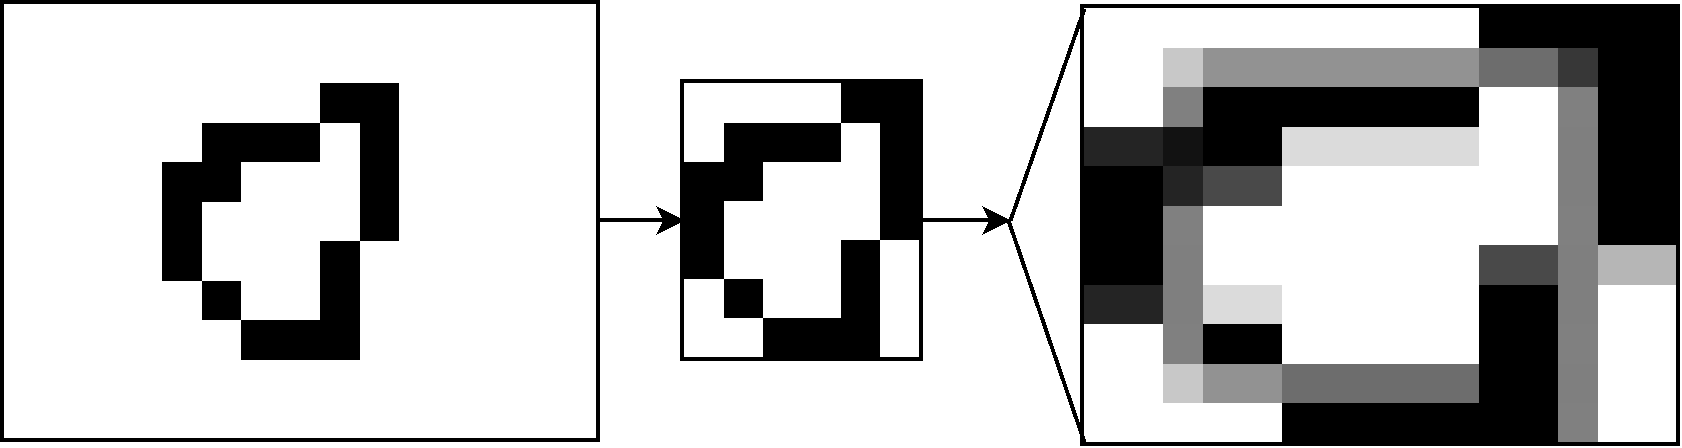
\includegraphics[width=10truecm]{images/crop_resize.png}
\caption{\textit{Symbol} előfeldolgozás}
\label{fig:symbol_pre}
\end{figure}

A mozdulat osztályozása utáni pillanatban a vásznat törölnünk kell, vagyis csupa 255 intenzitásértékkel kell ellátnunk, hogy a megszabott feltételek tovább ne teljesüljenek a további becsléseket elkerülve.

A modell betanításához képekre lesz szükségünk, amelyeket a programmal egyesével legyárthatunk és osztályozhatunk. További módszereket is használhatnánk a tanítóminta előállítására. Ilyenek lehetnek a minták generálása egy alap mintahalmazból zajosítással és egyéb megoldásokkal. Amint a minta rendelkezésünkre áll, a modell tanítható is.

A levegőben leírt gesztusok felismerése egy izgalmas kutatási terület, az általam elkészíett \textit{Optical Flow} megoldáson kívül is léteznek megközelítései. Általában a videófolyamon valamilyen szűrési technika segítségével kiemelik a megfigyelendő objektumot, valamilyen tulajdonsága alapján és a szűrt adatokon végzik el a további feldolgozási lépéseket. A szűrés történhet textúra, alak, mozgás, szín alapján is. \cite{fadhil2018trackingsurvey} Esetemben a mozgás alapján szerzett információk alapján történt a gesztus detektálása. A csupán mozgás alapú módszer hátrányai közé sorolhatjuk, bizonyos esetekben a pontatlanságot is, hiszen nincsen meghatározva pontosan a vizsgálandó objektum, így bármely megfigyelhető mozgásra képes aktiválódni. Viszont, más szemszögből nézve, ez a tulajdonság jelentheti a módszer előnyét is, hiszen így jobban alkalmazkodik a különböző bemenetekhez.

Kevert megoldásokkal is történhet a detektálás, például háttérmodell segítségével kivágott alak és a hozzátartozó elmozdulásértékek alapján rendkívül pontos gesztusfelismerő konstruálható. \cite{lin2009recognizing}

A gesztusfelismerést két csoportba sorolhatjuk: statikus és dinamikus. A statikus gesztusfelismerés alatt olyan megoldásokat értek, melyeknél nem játszik szerepet az idő. Vagyis például a detektálás a kézfej aktuális állása alapján történik. \cite{purohit2018precisehand} \cite{robust2017mouse} \cite{kumar2019calculator} Az ilyen típusú megközelítések nagy szerepet játszhatnak például a jelnyelv feldolgozásában is.

A dinamikus gesztusfelismerésnél az idő kulcs szerepet játszik. Az általam megalkotott módszer is ebbe a csoportba sorolható. Az ilyen megoldásokra jellemző, hogy a mozgást valamilyen módon rögzítik, különböző technikákkal lenyomatot készítenek a feldolgozás során kinyert adatok alapján és az így kapott mozgás képe alapján történik a detektálás. A mozgás rögzítése történhet a videó alapú megoldásokon kívül például gyroszkóppal ellátott speciális kesztyű segítségével is \cite{ponraj2012wireless}. Ha a videóalapú megoldásoknál maradunk, a csupán egy egyszerű kamera segítségével megvalósított megoldások viszonylag ritkák \cite{joseph2018visual}, az ilyen jellegű kutatásokhoz előszeretettel felhasználják a \textit{Kinect} kamerarendszert \cite{zhang2013new} \cite{tang2018structured}
Az dinamikus gesztusfelismerési módszerek jellemző alkalmazási területe a levegőbe írt karakterek/szimbólumok felismerése.

Természetesen mindegyik megoldásnak léteznek előnyei és egyben hátrányai is. Belátható, hogy univerzális megoldást találni a problémára nem lehet. Mérlegelni kell a rendelkezésünkre álló technikai lehetőségeinket és a felhasználási területből adódó igényeket is a használandó technika megválasztásánál.
